
\begin{kd}
	Trong công nghiệp, đơn chất nitrogen kết hợp với hydrogen tạo thành ammonia là một hợp chất quan trọng trong sản xuất phân bón, hoá chất.\\
	Tại sao phản ứng trên cấn thực hiện ở nhiệt độ cao? Đơn chất nitrogen đóng vai trò gì trong phản ứng đó?
\end{kd}
\subsubsection{Trạng thái tự nhiên}
		Nitơ (N) là một nguyên tố hóa học có số hiệu nguyên tử là 7. Đây là một trong những phi kim quan trọng nhất trong tự nhiên và đóng vai trò không thể thiếu trong chu trình sinh địa hóa học.Nitơ tồn tại dưới nhiều dạng và có mặt trong nhiều hệ sinh thái khác nhau, từ khí quyển, đại dương đến các hệ sinh vật sống. Dưới đây là các nguồn phân bố chính của nitơ:
	\clearpage
	\begin{itemize}
		\item \indam[black]{Nitơ trong khí quyển}:
			\begin{paracol}{2}
				\begin{itemize}
					\item Nitơ tồn tại chủ yếu dưới dạng nitơ phân tử (N$_2$), là một chất khí không màu, không mùi.
					\item N$_2$ khá trơ về mặt hóa học do liên kết ba rất bền giữa các nguyên tử nitơ trong phân tử N$_2$.
					\item Khí Nitơ chiếm khoảng 78\% thành phần khí quyển.
				\end{itemize}
				\switchcolumn
				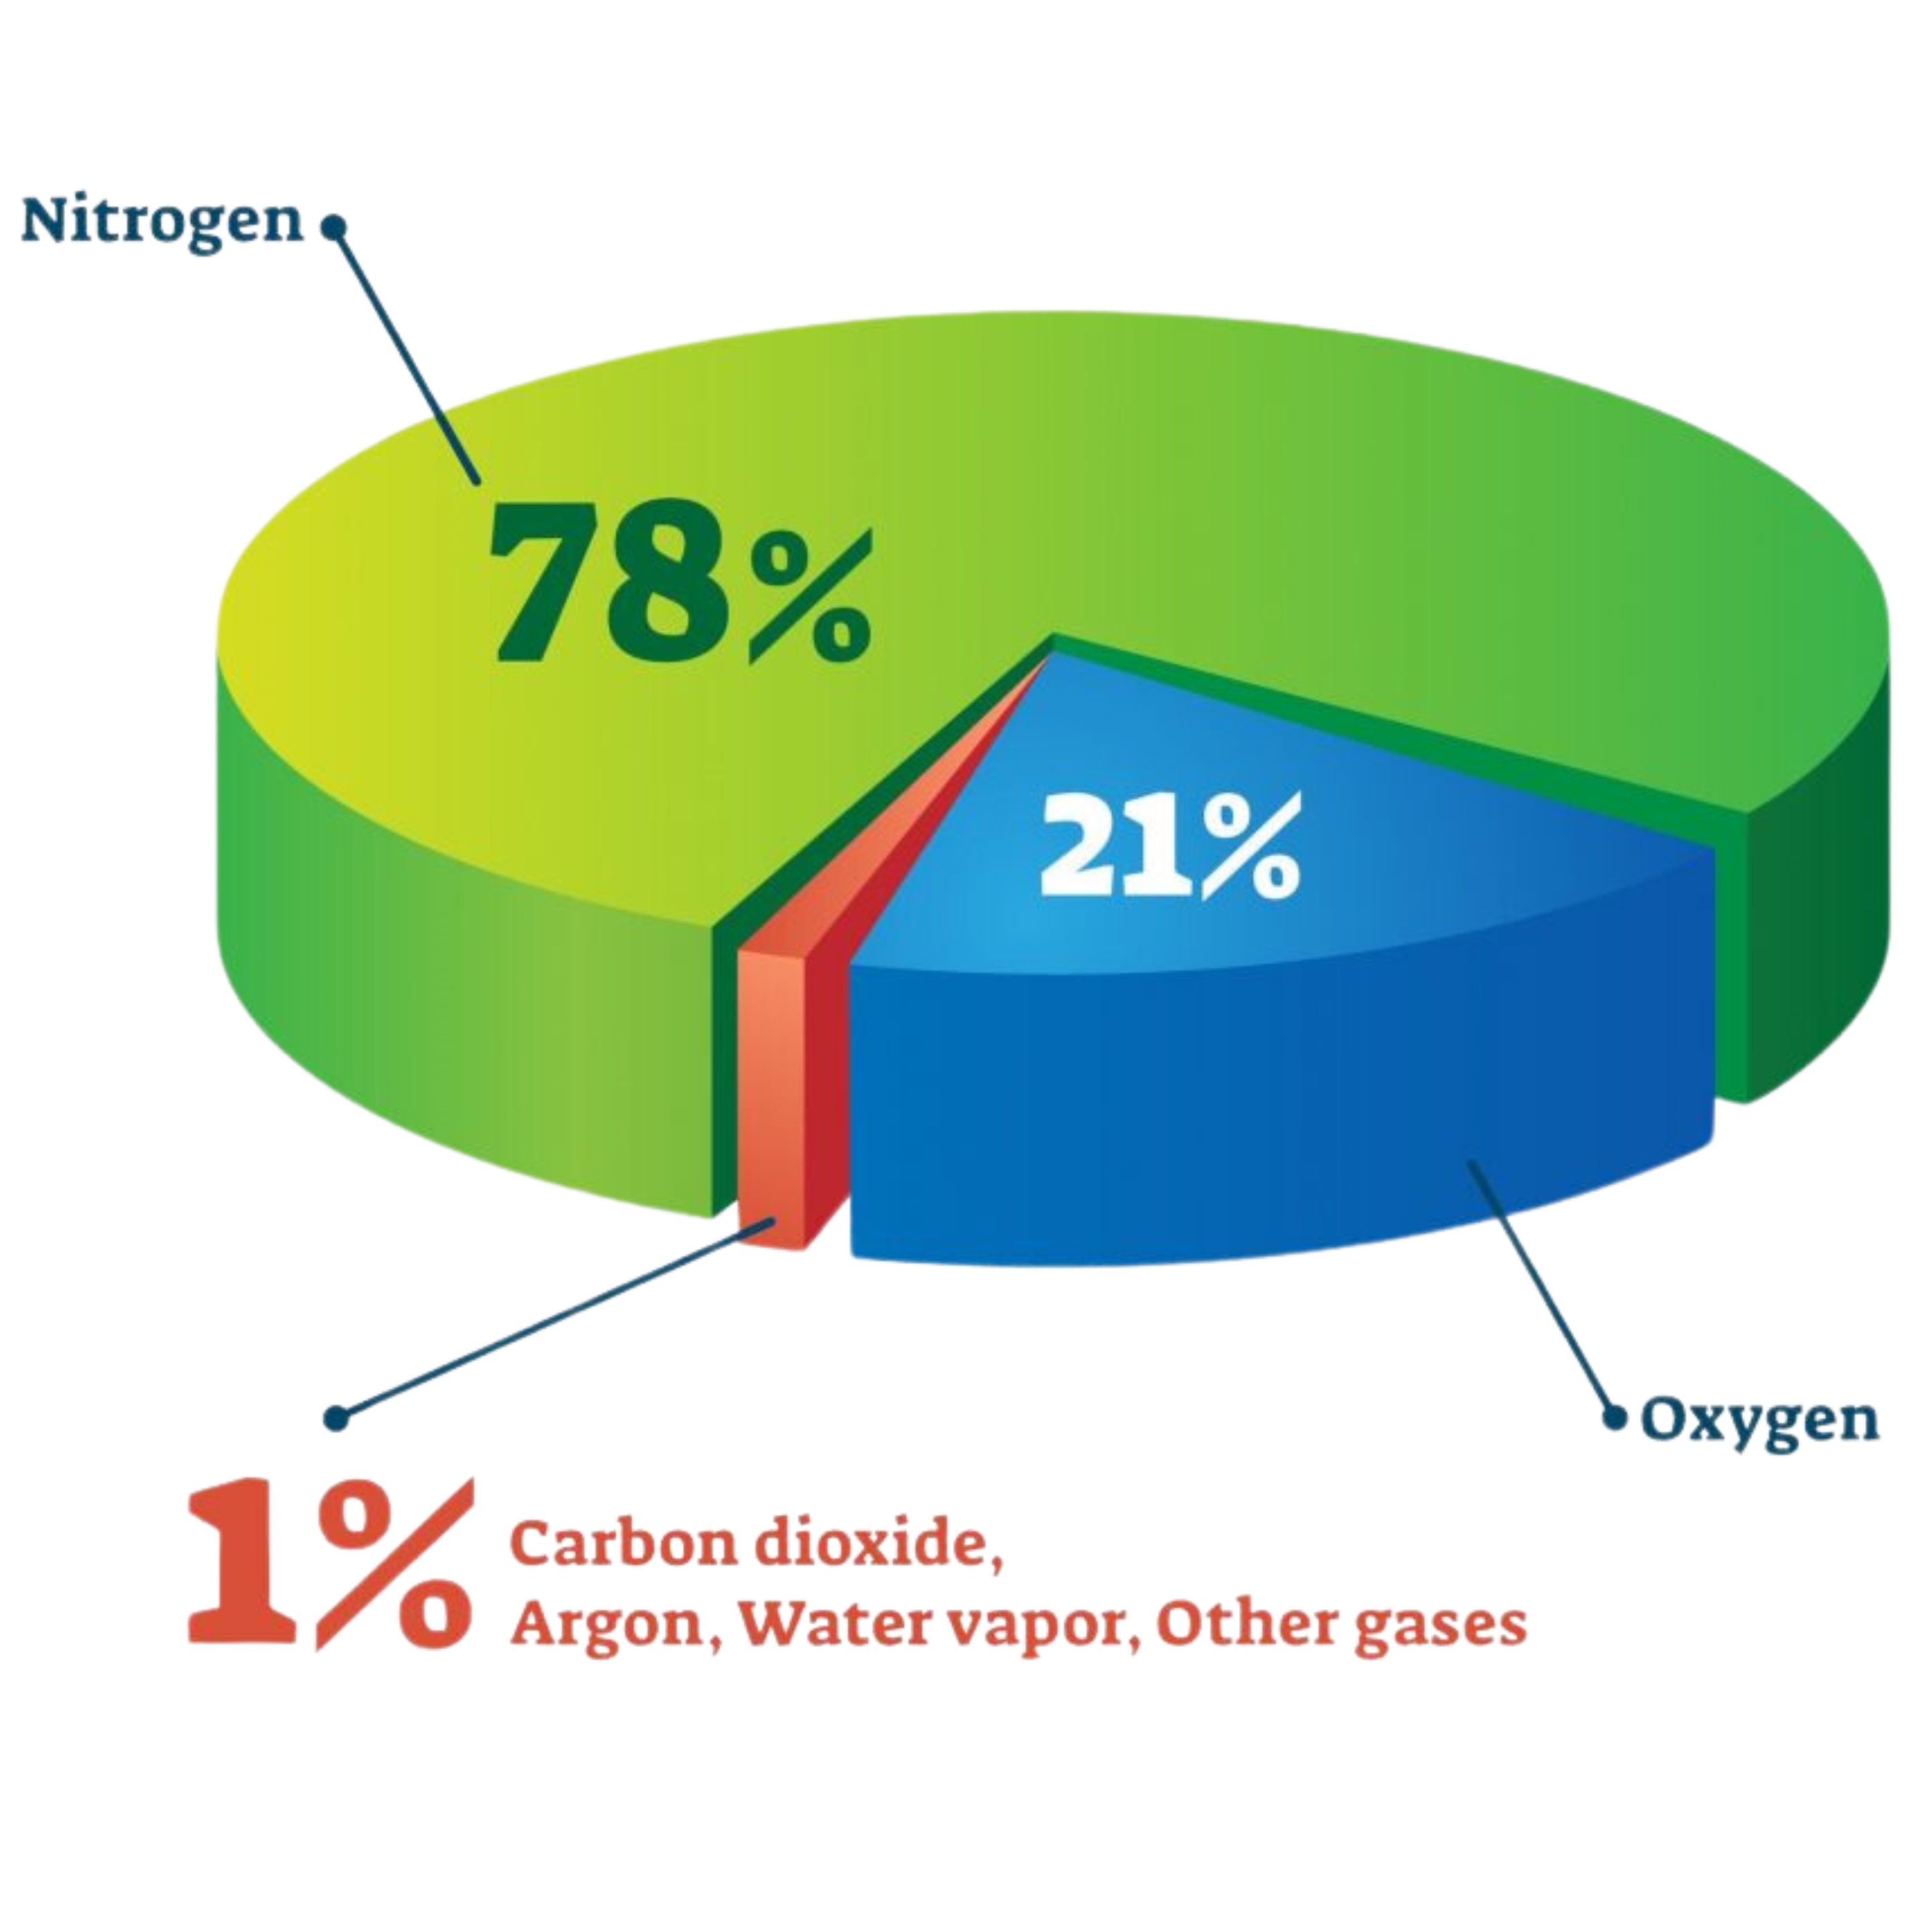
\includegraphics[height=4cm]{Images/anhhoa11/ThanhphanKhongKhi.png}
				\captionof{figure}{Thành phần thể tích\\ của không khí}
			\end{paracol}
		\begin{paracol}{2}
			\item \indam[black]{Nitơ trong sinh vật sống:} 
			\begin{itemize}
				\item Nitơ là thành phần thiết yếu của các axit amin, protein và axit nucleic.
				\item Trong hệ sinh học, Nitơ thường tồn tại dưới dạng amonia (NH$_3$), nitrit (NO$_2^-$), và nitrat (NO$_3^-$).
				\item Nitơ có vai trò quan trọng trong sự phát triển của thực vật và chu trình dinh dưỡng.
			\end{itemize}
			\switchcolumn
			\begin{Bancobiet}[\mycolor]
				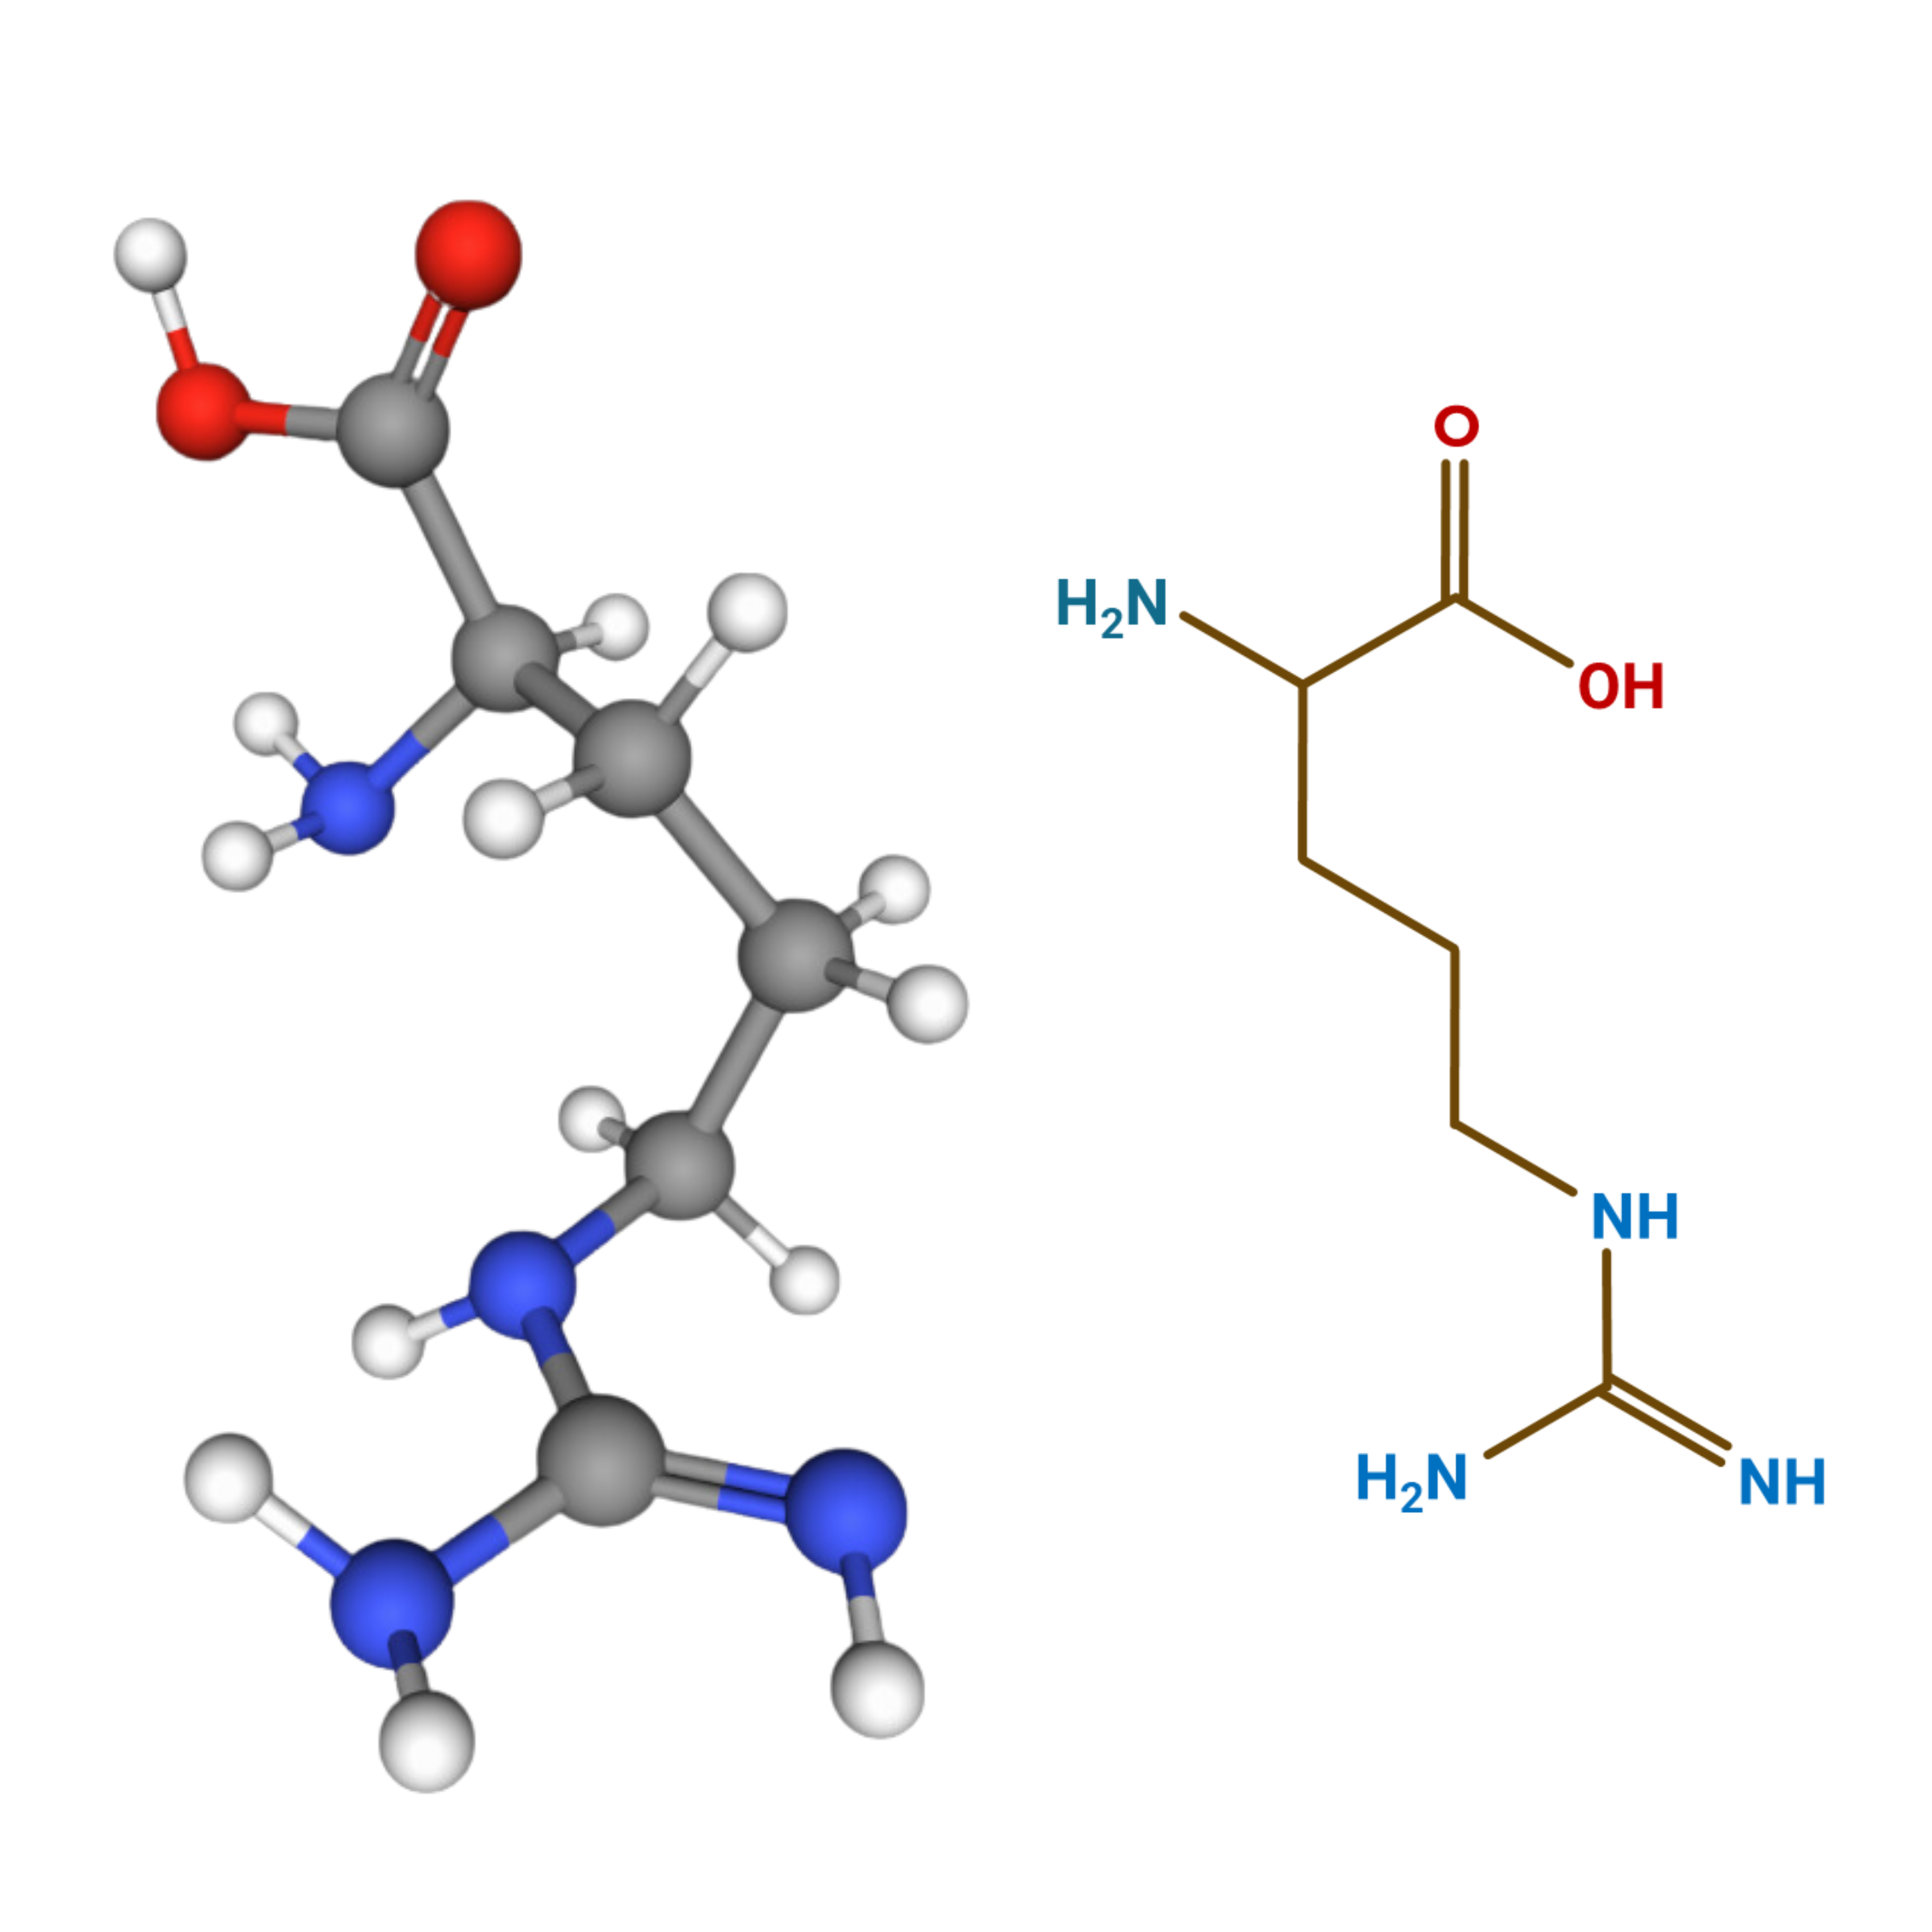
\includegraphics[width=5cm,trim={2cm 2cm 0.5cm 2cm},clip]{Images/anhhoa11/HopchatchuaNito.png}
				Arginine là chất thiết yếu cho quá trình tổng hợp protein trong cơ thể.
				Phân tử arginine chứa 4 nguyên tử $N$.
			\end{Bancobiet}
		\end{paracol}
		\begin{paracol}{2}
				\item \indam[black]{Nitơ trong đất:} 
				\begin{itemize}
					\item Nitơ trong đất chủ yếu tồn tại dưới dạng các hợp chất vô cơ như amonia (NH$_3$) và nitrat (NO$_3^-$).
					\item Thực vật hấp thụ nitrat và amonia từ đất để tổng hợp protein và các hợp chất hữu cơ khác.
				\end{itemize}
				\item \indam[black]{Nitơ trong các đại dương:} 
				\begin{itemize}
					\item Đại dương chứa một lượng lớn nitơ, chủ yếu tồn tại dưới dạng các ion nitrat và amonia.
					\item Nitơ đóng vai trò quan trọng trong hệ sinh thái biển, hỗ trợ sự phát triển của sinh vật phù du và các sinh vật khác.
				\end{itemize}
				\switchcolumn
				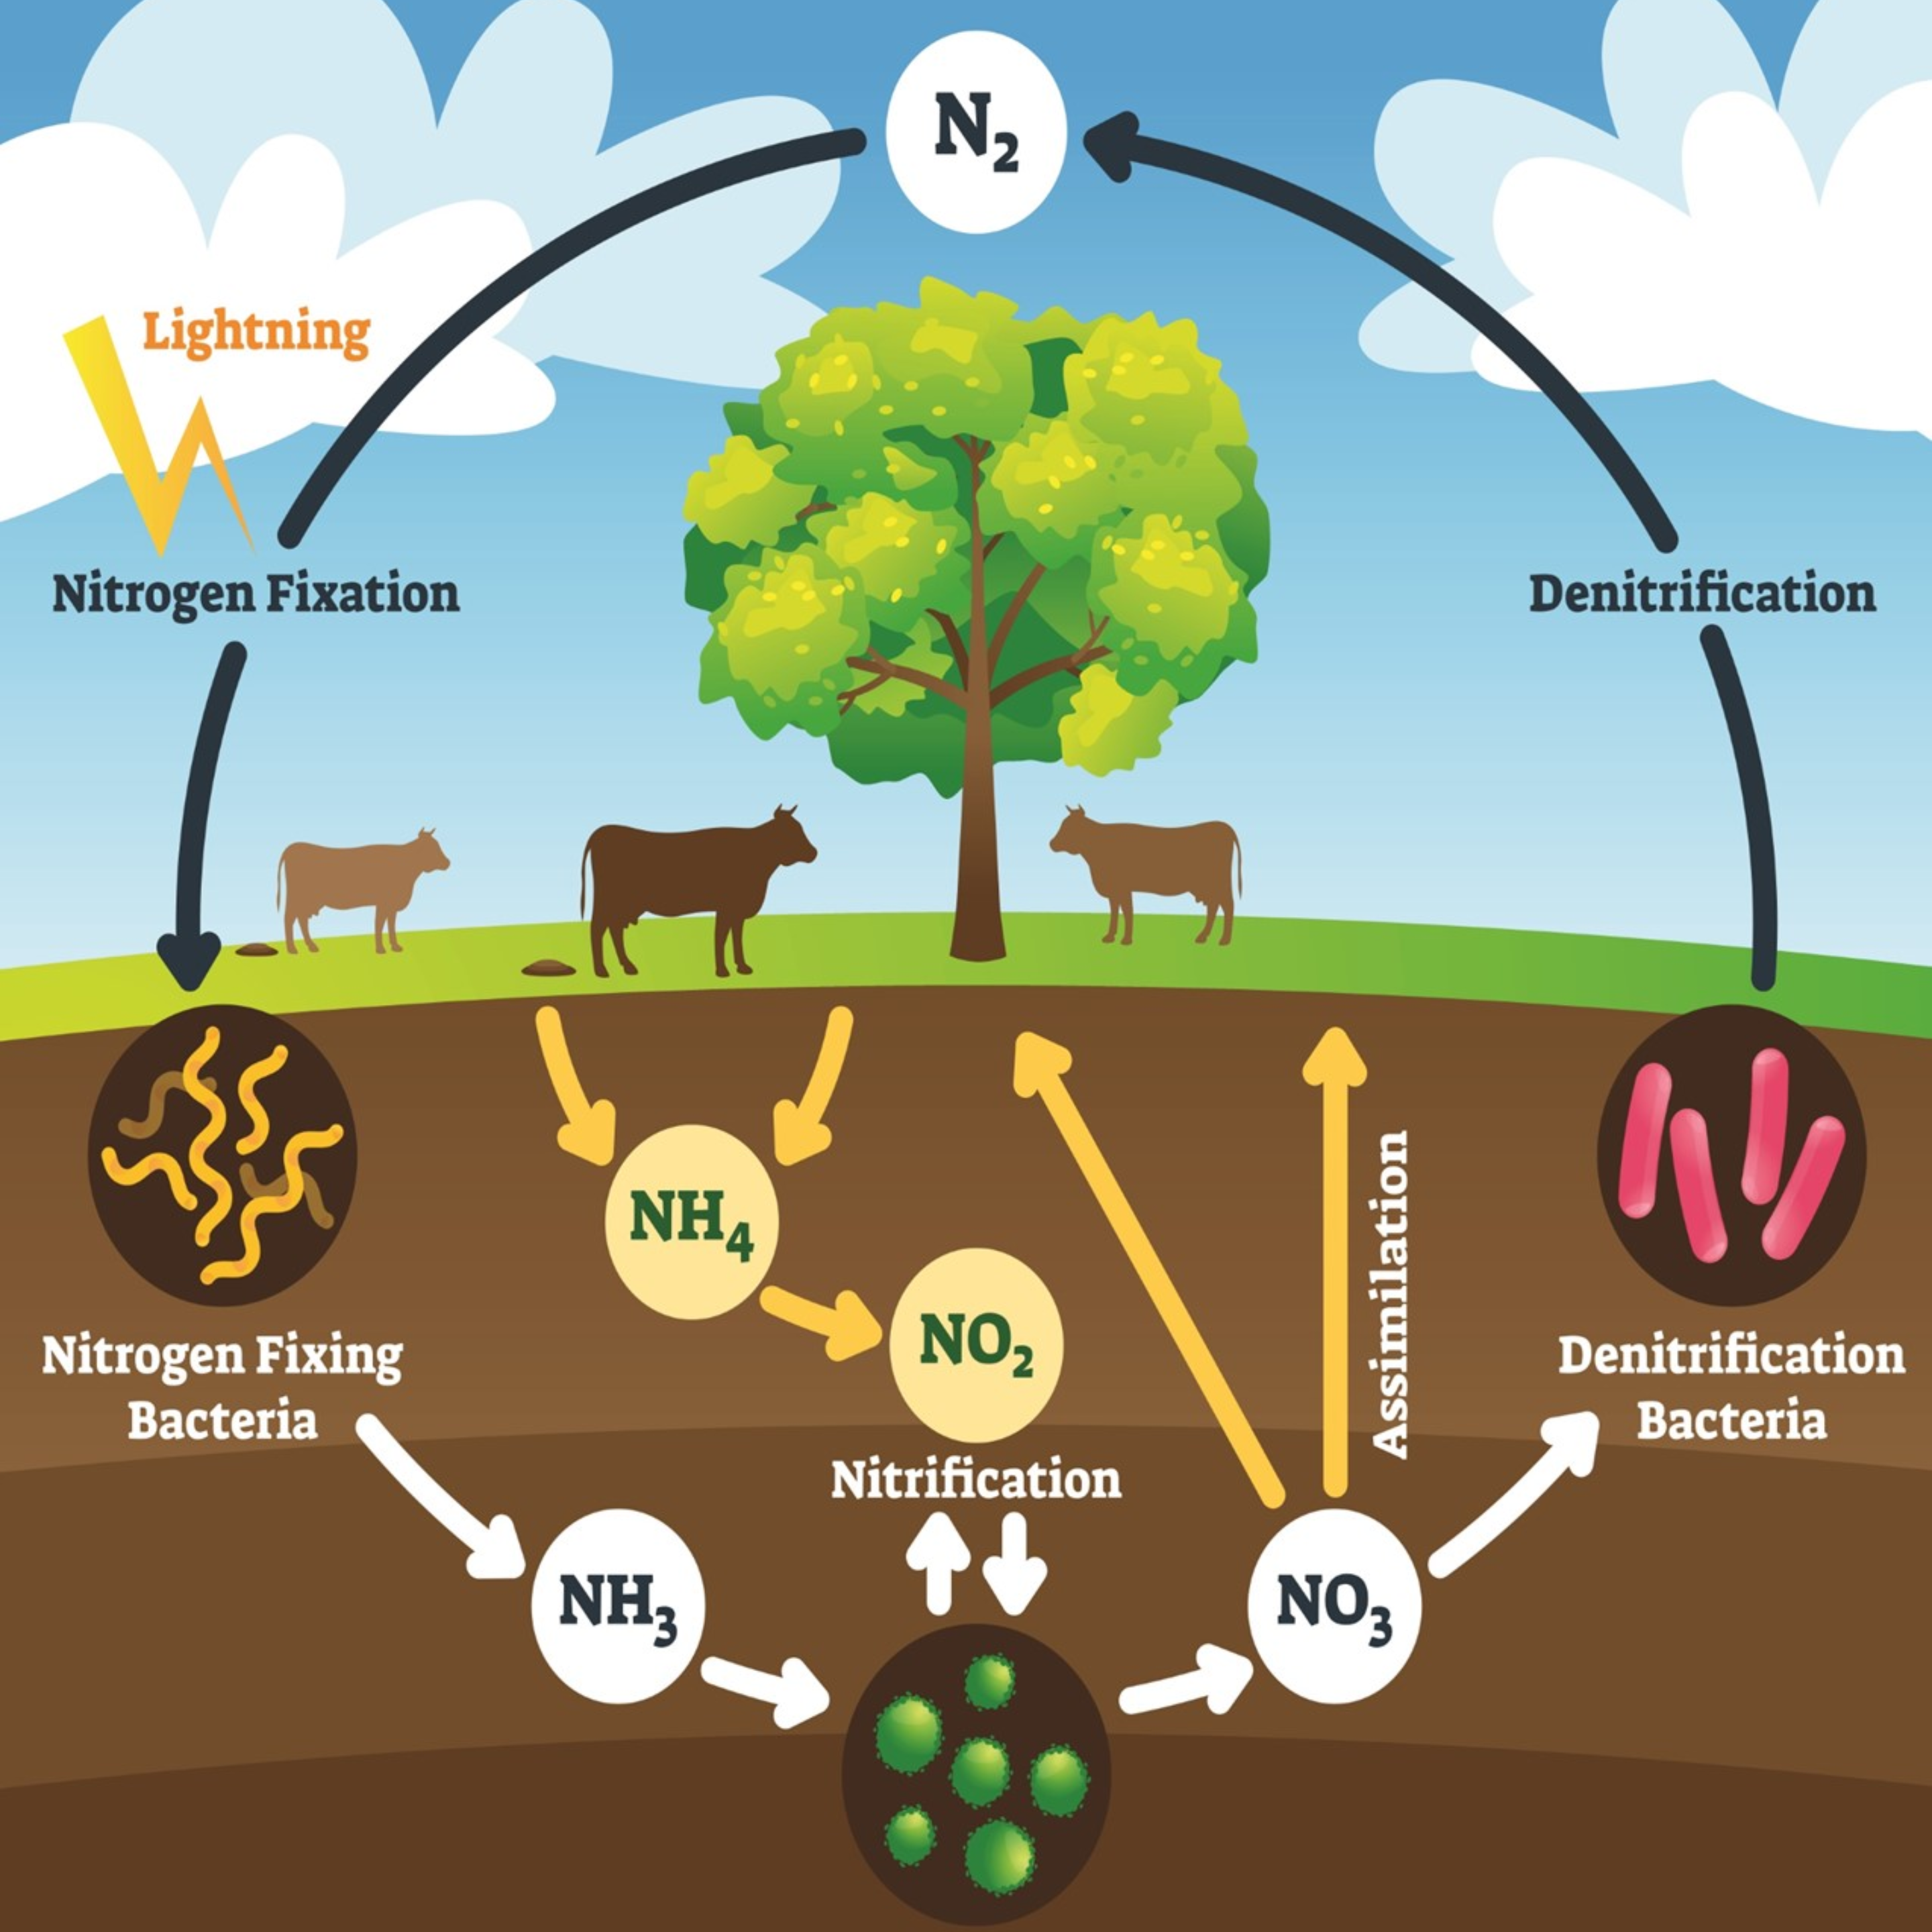
\includegraphics[width=5cm]{Images/anhhoa11/ChutrinhNitrogen.png}
		\end{paracol}
	\end{itemize}
\subsubsection{Cấu tạo nguyên tử, phân tử}
	\Noibat[][]{Cấu tạo nguyên tử}
	\begin{hopdongian}
		\hinhphai{Nguyên tố nitrogen ở ô số 7 , nhóm VA, chu kì 2 trong bảng tuần hoàn. Nguyên tử nitrogen có độ âm điện lớn $(3,04)$. Nitrogen là phi kim điển hình.\\
		Nitrogen tạo ra nhiều hợp chất với các số oxi hoá khác nhau từ -3 đến +5 . Các số oxi hoá thường gặp của nitrogen được biểu diễn ở trục số oxi hoá dưới đây.\\
		\begin{tikzpicture}[declare function={r=3;},line cap=round,line join=round]
			\foreach \x [count=\i from 1] in {-3,0,1,2,3,4,5}{%
				\path (\x,0) node [inner sep=0pt,outer sep =0pt,anchor =center] (d-\i){%
					\tikz{%
						\draw[line width=1pt,\maunhan](0,0) --(0,4pt);
					}
				};
				\path (d-\i.north) node [anchor=south,text=\maudam,font=\bfseries\sffamily\scriptsize] {%
					\ifnum\x>0
					+\x
					\else
					\x
					\fi
				};
			}
			\draw[->,-stealth,line width=0.8pt](-3.5,0)--(5.5,0);
			\path (d-2.south) node [anchor=north,text=\maunhan,font=\large] {$\mathsf{N_2}$};
		\end{tikzpicture}
		}{%
			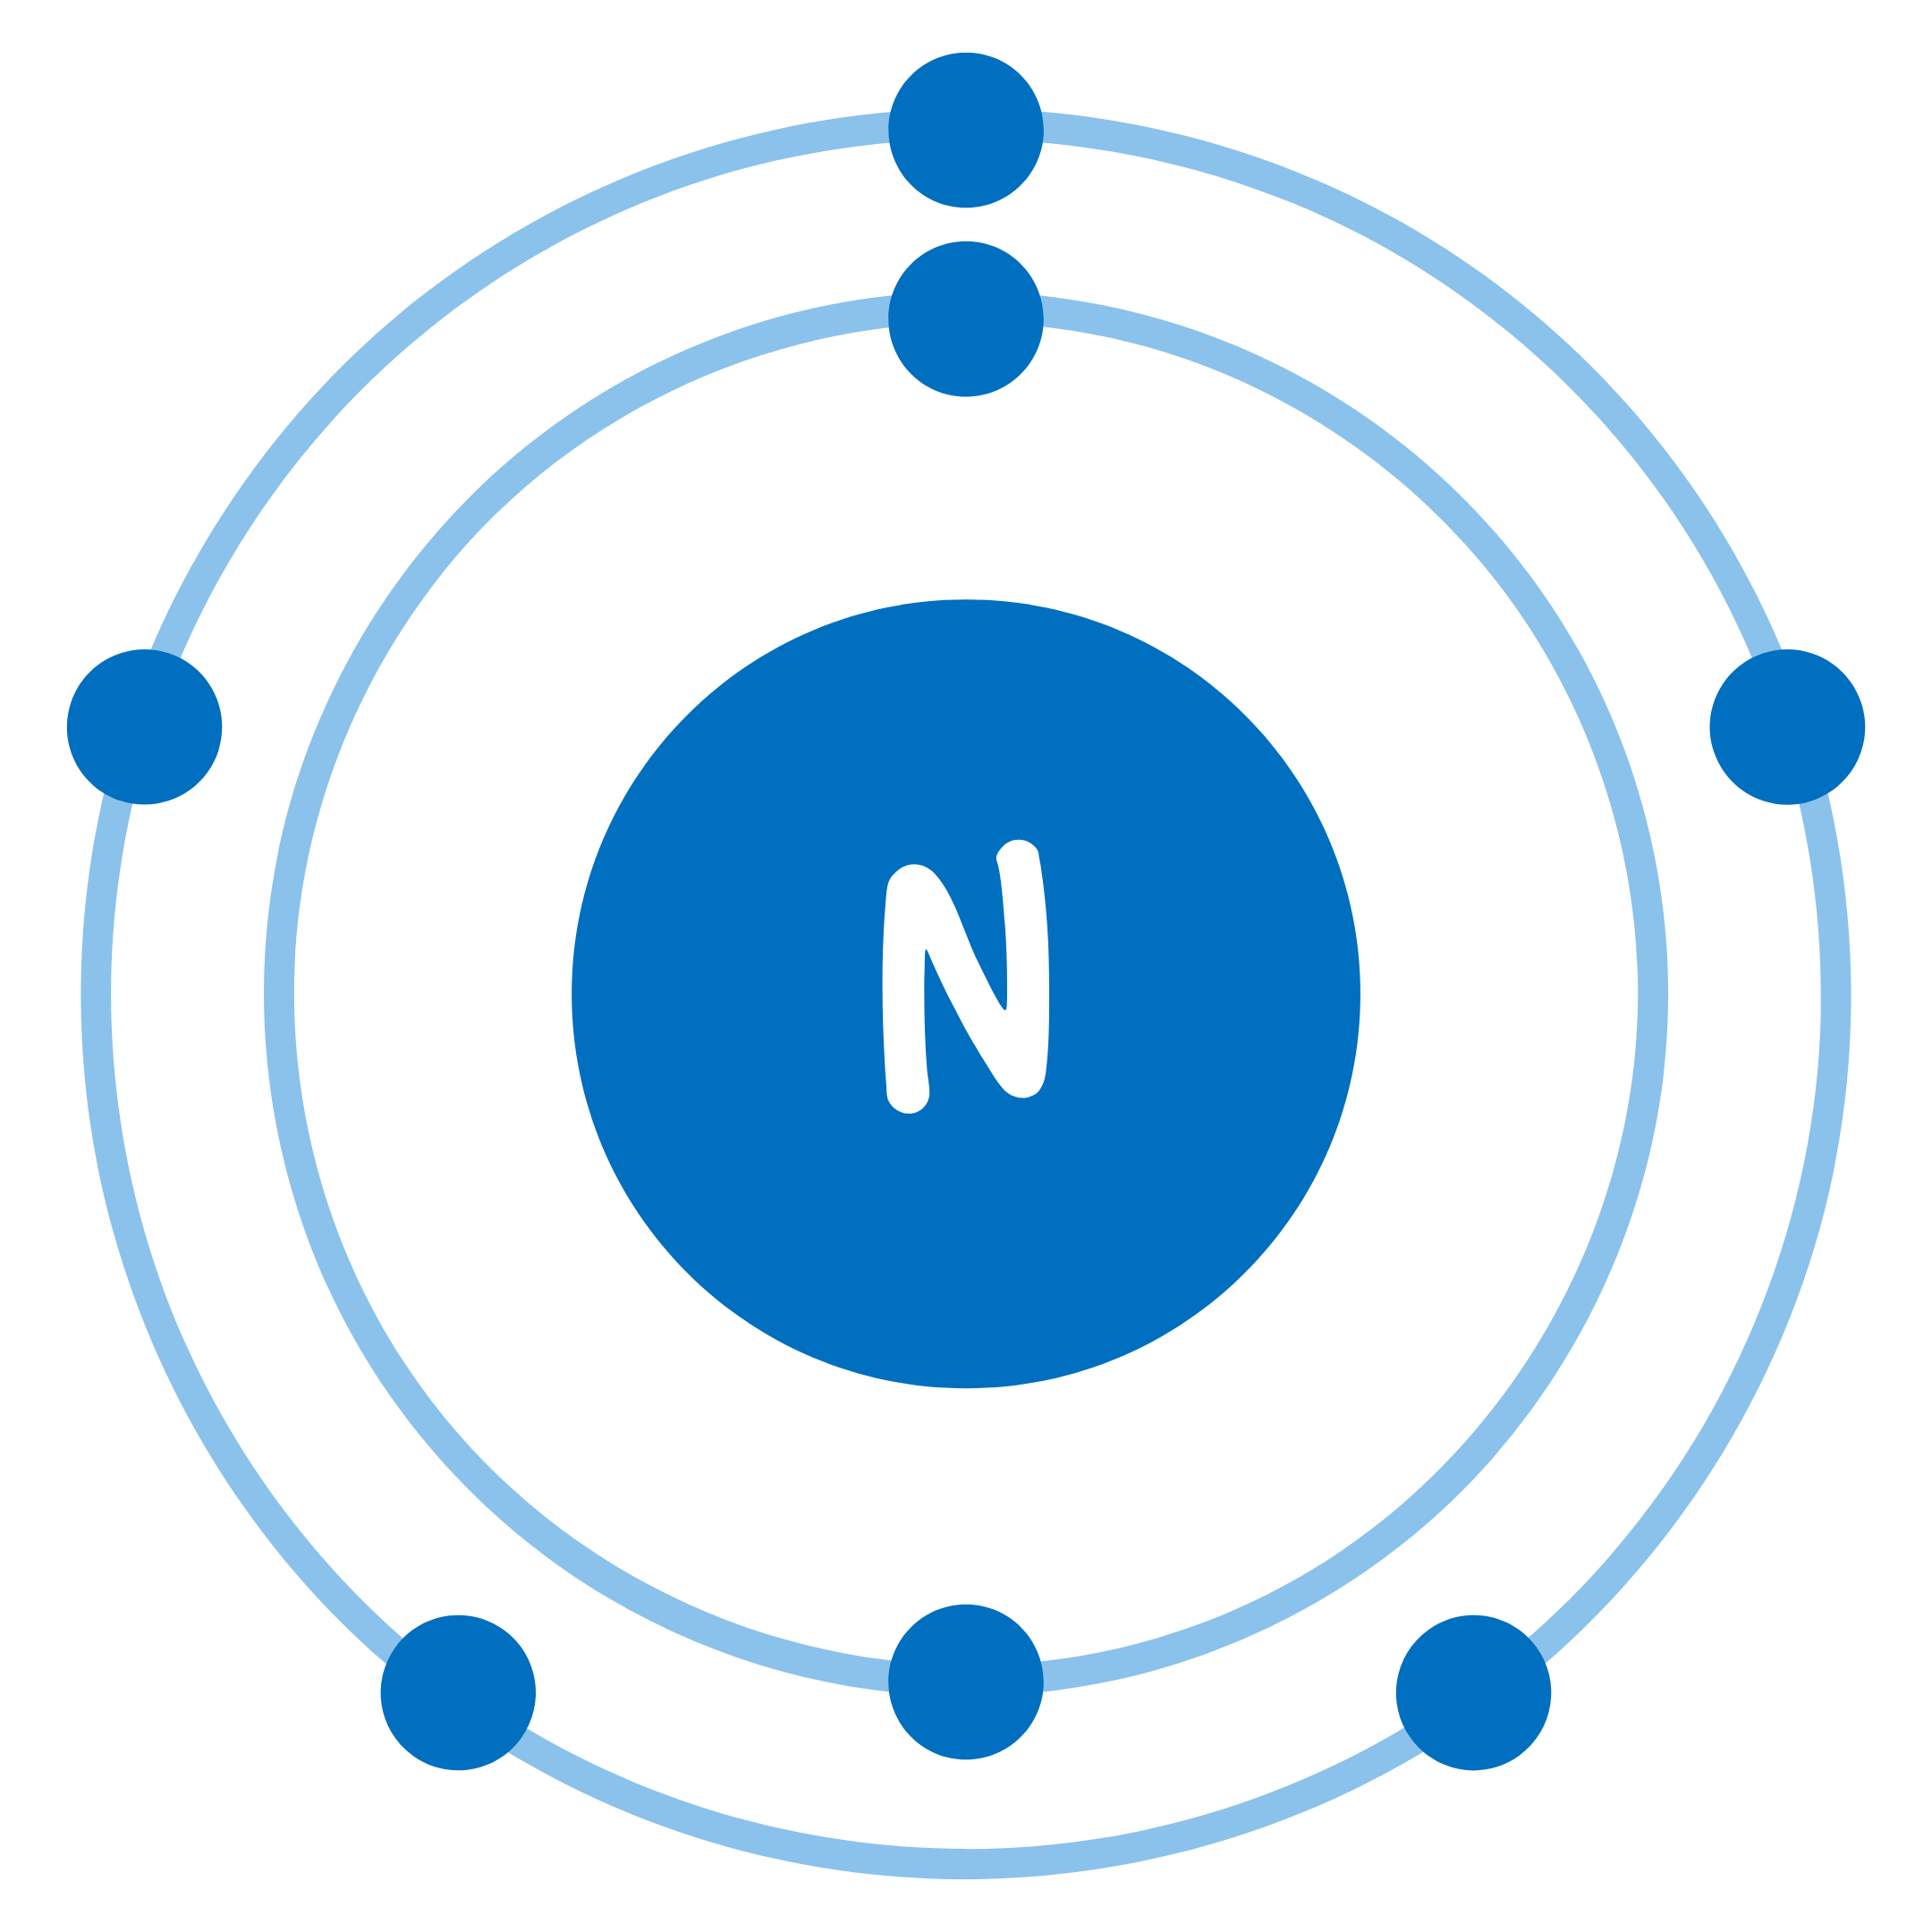
\includegraphics[width=4cm]{Images/anhhoa11/SodocautaoNito.png}
		}
	\end{hopdongian}
	\begin{hoivadap}
		\begin{cauhoi}
			\item Sắp xếp các hợp chất sau vào vị trí tương ứng trong trục biểu diễn số oxi hoá của nitrogen: $\mathrm{NO}, \mathrm{N}_2 \mathrm{O}, \mathrm{NO}_2, \mathrm{NH}_3, \mathrm{HNO}_2, \mathrm{HNO}_3, \mathrm{NH}_4 \mathrm{Cl}, \mathrm{KNO}_2, \mathrm{NaNO}_3$.
			\item Dựa vào trục biểu diễn số oxi hoá của nitrogen để giải thích nitrogen có cả tính oxi hoá và tính khử. Viết một quá trình oxi hoá và một quá trình khử để minh hoạ.
		\end{cauhoi}
		\loigiai{
		\begin{cauhoi}
			\item \begin{tikzpicture}[declare function={r=3;hs=1.5;},line cap=round,line join=round, baseline]
				\foreach \x [count=\i from 1] in {-3,0,1,2,3,4,5}{%
					\path (\x*hs,0) node [inner sep=0pt,outer sep =0pt,anchor =center] (d-\i){%
						\tikz{%
							\draw[line width=1pt,\maunhan](0,0) --(0,4pt);
						}
					};
					\path (d-\i.north) node [anchor=south,text=\maudam,font=\bfseries\sffamily\scriptsize] {%
						\ifnum\x>0
						+\x
						\else
						\x
						\fi
					};
				}
				\draw[->,-stealth,line width=0.8pt](-3.5*hs,0)--(5.5*hs,0);
				\foreach \x/\n in {%
					1/{$NH_3$, $NH_4Cl$},3/$N_2O$,
					4/$NO$,5/{$HNO_2$, $KNO_2$},
					6/{$NO_2$},7/{$HNO_3$, $NaNO_3$}
					}{
					\path (d-\x.south) node [anchor=north,text=\maunhan,font=\scriptsize,fill=\maunhan!15,inner sep=4pt, outer sep =2pt,rounded corners =3pt] {\n};
				}
				\path (d-2.south) node [anchor=north,text=\maudam,font=\large,fill=\maudam!15,inner sep=4pt, outer sep =2pt,rounded corners =3pt] {$\mathsf{N_2}$};
			\end{tikzpicture}
			\item $N_2$ có số oxi-hóa bằng $0$ là số oxi hóa trung gian nên khi tham gia phản ứng hóa học $N_2$ sẽ có 2 khuynh hướng:
			\begin{itemize}
				\item giảm số oxi-hóa từ $0$ xuống $-3$ thể hiện tính oxi hóa:
				\textbf{Ví dụ:}  $N_2$ $+$ $H_2$ $\xleftrightarrow$ $NH_3$
				\item tăng số oxi-hóa từ $0$ lên $+1$, $+2$, $+3$, $+4$, $+5$ thể hiện tính khử:\textbf{Ví dụ:}  $N_2$ $+$ $O_2$ $\xrightarrow[$3000^\circ C$][][1.5]$ $2NO$
			\end{itemize}
		\end{cauhoi}
		}
	\end{hoivadap}
	\Noibat[][]{Cấu tạo phân tử}
	\immini{Phân tử nitrogen gồm hai nguyên tử, liên kết với nhau bằng liên kết ba ( 1 liên kết $\sigma$ và 2 liên kết $\pi)$. Phân tử nitrogen có năng lượng liên kết lớn $(945 \mathrm{~kJ} / \mathrm{mol})$ và không có cực.}{
		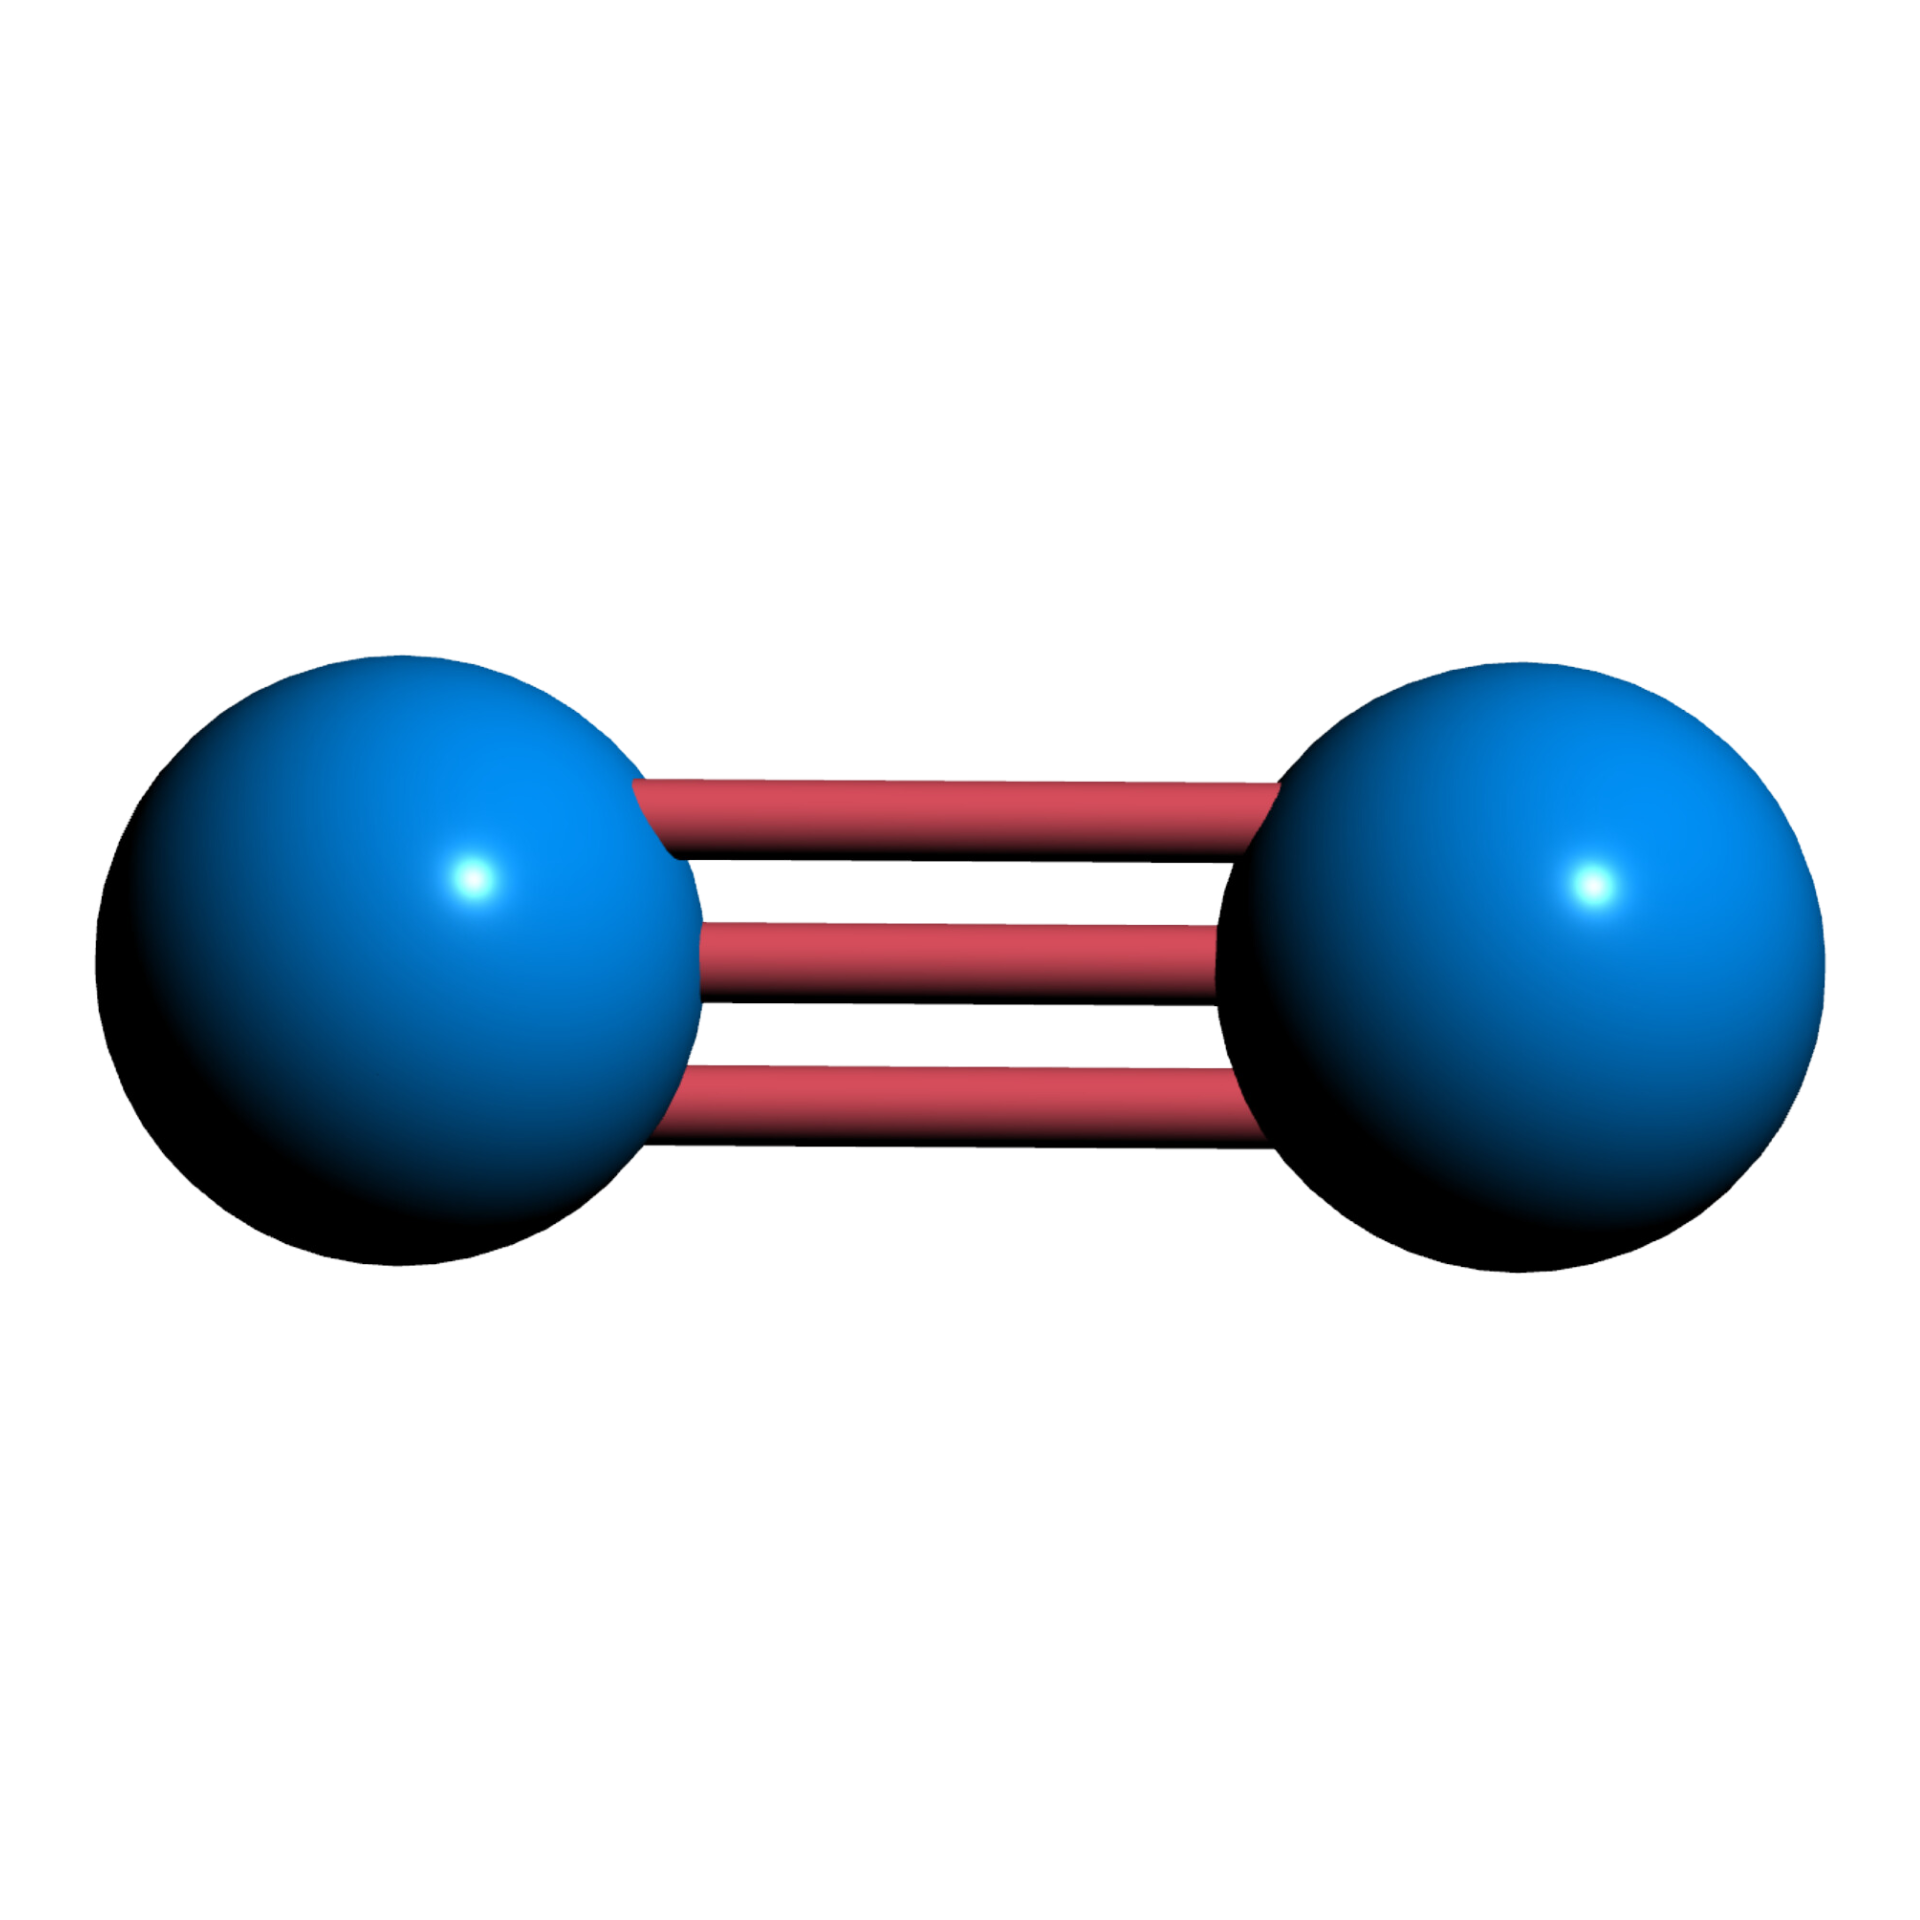
\includegraphics[width=5cm]{Images/anhhoa11/CautaoPTNito.png}
	}
	\begin{hoivadap}
		\begin{cauhoi}
			\item Viết công thức electron, công thức Lewis và công thức cấu tạo của phân tử nitrogen.
			\item Từ cấu tạo phân tử, hãy cho biết tại sao phân tử $N_2$ có năng lượng liên kết lớn. Dự đoán về khả năng hoạt động hoá học của nitrogen ở nhiệt độ thường.
		\end{cauhoi}
		\loigiai{%
		\begin{cauhoi}
			\item \begin{tabular}{C{0.2\linewidth}C{0.2\linewidth}C{0.2\linewidth}}
			Công thức electron&Công thức Lewis&Công thức cấu tạo\\
			\chemfig[atom sep=2em]{\charge{90:2pt=\:,0:2pt=\.,0:2pt=\.[{.style={yshift=2.65mm,fill=black}}],0:2pt=\.[{.style={yshift=-2.65mm,fill=black}}]}{N}-[,0.85,,,draw=none]\charge{90:2pt=\:,180:2pt=\.,180:2pt=\.[{.style={yshift=2.65mm,fill=black}}],180:2pt=\.[{.style={yshift=-2.65mm,fill=black}}]}{N}}&\chemfig[atom sep=2em]{\charge{90:2pt=\:}{N}~\charge{90:2pt=\:}{N}}&\chemfig[atom sep=2em]{N~N}
			\end{tabular}
			\item Do trong cấu tạo có liên kết ba bền vững nên năng lượng liên kết rất lớn vì thế ở nhiệt độ thường phân tử $N_2$ khá trơ về mặt hóa học.
		\end{cauhoi}
		}
	\end{hoivadap}
\subsubsection{Tính chất vật lý}
	\begin{ghinho}
		\Rightpicture[0.65]{Ở điều kiện thường, nitrogen là chất khí, không màu, không mùi, không vị, khó hoá lỏng (hoá lỏng ở $-196^{\circ} \mathrm{C}$ ), tan rất ít trong nước (1 lít nước hoà tan được 0{,}012 lít khí nitrogen). Khí nitrogen không duy trì sự cháy và sự hô hấp.}{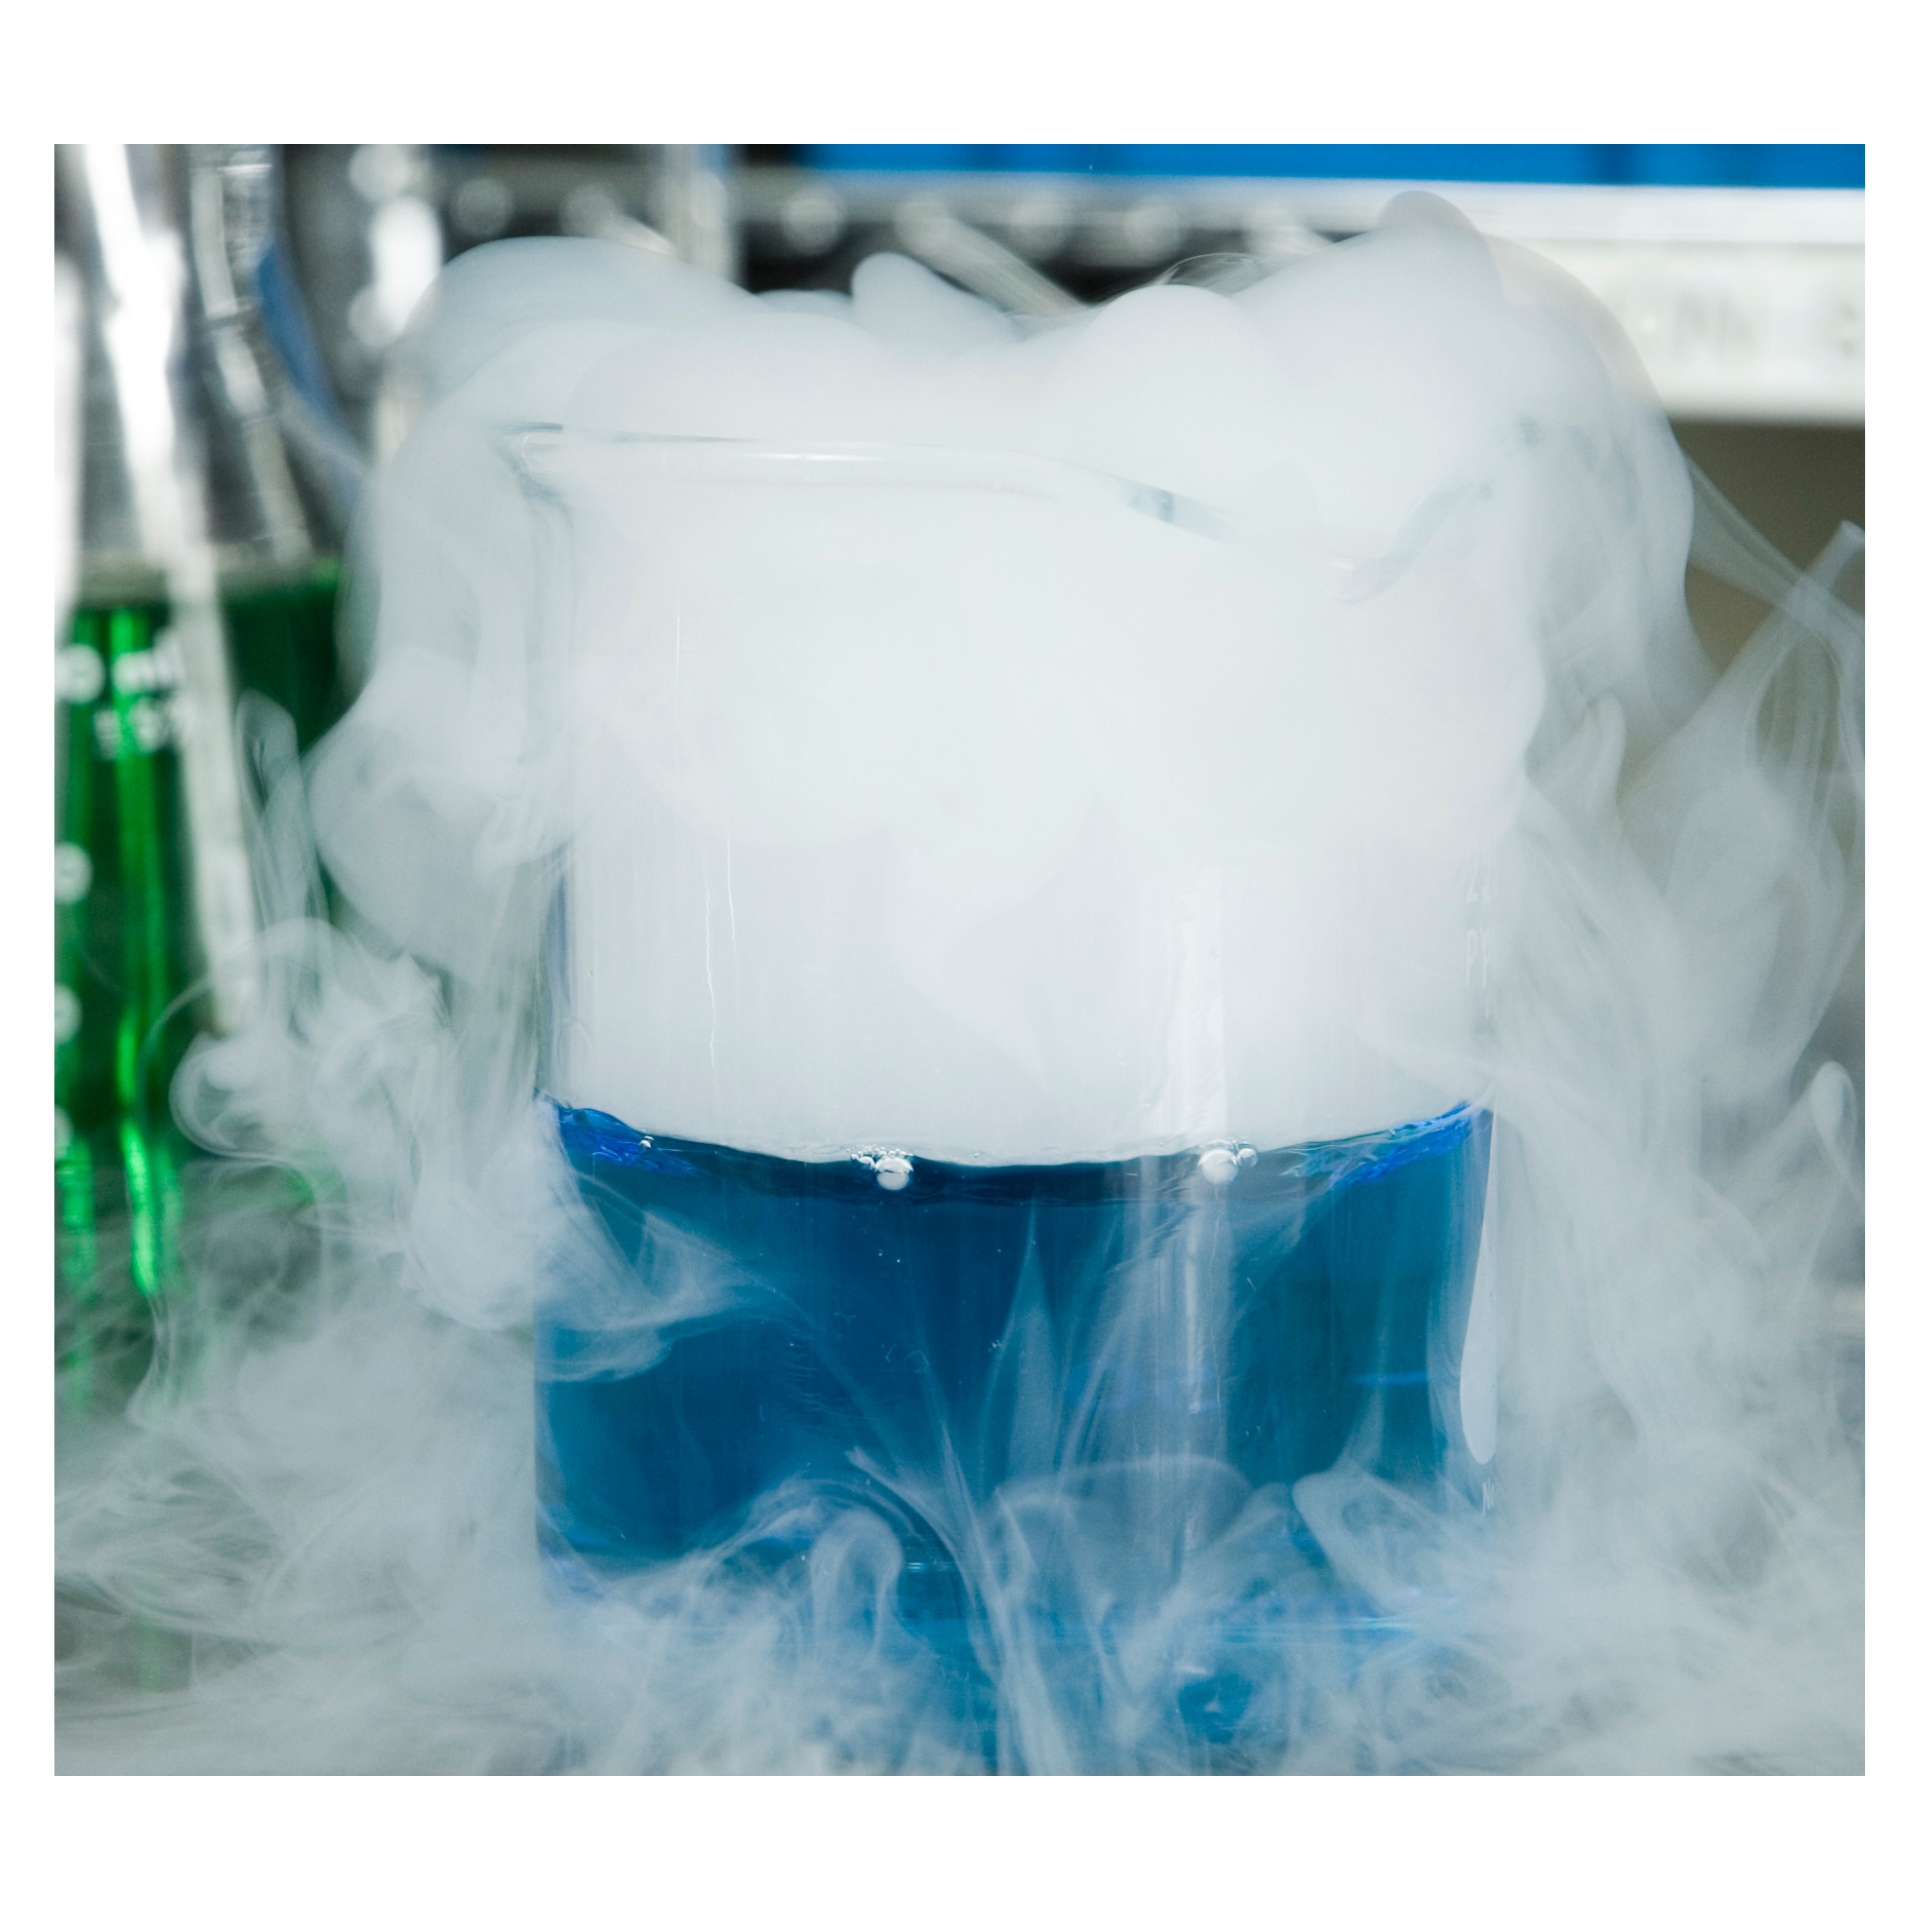
\includegraphics[width=5cm]{Images/anhhoa11/Liquid_Nitrogen.png}}
	\end{ghinho}
	\begin{hoivadap}
		\begin{cauhoi}
			\item Dựa vào tương tác van der Waals, hãy giải thích tại sao đơn chất $\mathrm{N}_2$ khó hoá lỏng và ít tan trong nước.
		\end{cauhoi}
		\loigiai{
		\begin{itemize}
			\item Do phân tử $N_2$ không phân cực, khối lượng nhỏ  nên lực tương tác van der Waals giữa các phân tử với nhau rất nhỏ dẫn đến lực hút giữa các phân tử  không thể vượt qua động năng lúc này các phân tử dễ dàng chuyển động ra xa nhau , duy trì trạng thái khí.
			\item Vì $N_2$ là phân tử phân cực trong khi đó $H_2O$ là một phân tử phân cực nên tương tác van der Waals giữa $H_2O$ và $N_2$ yếu nên $N_2$ ít tan trong nước.
		\end{itemize}
			}
	\end{hoivadap}
\subsubsection{Tính chất hóa học}
 $\mathrm{N}_2(\mathrm{g})+3 \mathrm{H}_2(\mathrm{g}) \xharpoonarrow[$400 - 600 ^\circ$][$200~bar, Fe$][2] 2 \mathrm{NH}_3(\mathrm{g})$ $\Delta_{\mathrm{r}} \mathrm{H}_{298}^{\circ}=-91{,}8 \mathrm{~kJ}$
\subsubsection{Ứng dụng}